%# -*- coding: utf-8-unix -*-
%%==================================================

\chapter{写作示例}
\label{chap2}

\section{列表环境}

\subsection{无序列表}

以下是一个无序列表的例子,列表的每个条目单独分段。

\begin{itemize}
	\item 这是一个无序列表。
	\item 这是一个无序列表。
	\item 这是一个无序列表。
\end{itemize}

使用\verb+itemize*+环境可以创建行内无序列表。
\begin{itemize*}
	\item 这是一个无序列表
	\item 这是一个无序列表
	\item 这是一个无序列表
\end{itemize*}
行内无序列表条目不单独分段,所有内容直接插入在原文的段落中。

\subsection{有序列表}

使用环境\verb+enumerate+和\verb+enumerate*+创建有序列表,
使用方法无序列表类似。
\begin{enumerate}
	\item 这是一个有序列表。
	\item 这是一个有序列表。
	\item 这是一个有序列表。
\end{enumerate}

使用\verb+enumerate*+环境可以创建行内有序列表。
\begin{enumerate*}
	\item 这是一个默认有序列表
	\item 这是一个默认有序列表
	\item 这是一个默认有序列表
\end{enumerate*}
行内有序列表条目不单独分段,所有内容直接插入在原文的段落中。

\subsection{描述列表}
使用环境\verb+description+可创建带有主题词的列表,条目语法是\verb+\item[主题] 内容+。
\begin{description}
	\item[主题一] 详细内容
	\item[主题二] 详细内容
	\item[主题三] 详细内容 \ldots
\end{description}

\section{数学排版}

\subsection{公式排版}

这里有举一个长公式排版的例子,来自\href{http://www.tex.ac.uk/tex-archive/info/math/voss/mathmode/Mathmode.pdf}{《Math mode》}:

\begin {multline}
\frac {1}{2}\Delta (f_{ij}f^{ij})=
2\left (\sum _{i<j}\chi _{ij}(\sigma _{i}-
\sigma _{j}) ^{2}+ f^{ij}\nabla _{j}\nabla _{i}(\Delta f)+\right .\\
\left .+\nabla _{k}f_{ij}\nabla ^{k}f^{ij}+
f^{ij}f^{k}\left [2\nabla _{i}R_{jk}-
\nabla _{k}R_{ij}\right ]\vphantom {\sum _{i<j}}\right )
\end{multline}

\subsection{SI单位}

使用\verb+siunitx+宏包可以方便地输入SI单位制单位,例如\verb+\SI{5}{\um}+可以得到\SI{5}{\um}。

\subsection{定理环境}

在这个模板中,定义了如下几个环境
remark(注),mythm(定理),myprop(性质),mydef(定义),example(例)。
amsmath还提供了一个proof(证明)的环境。
我们举例说明它们的用法。

注环境
\begin{remark}
	存在事先给定的一系列基本操作,并且这些基本操作永远不会改变。
\end{remark}
\begin{remark}
	每个操作都可逆。
	\label{o1.2}
\end{remark}
\begin{remark}
	每一个操作都是确定性的。
\end{remark}
\begin{remark}
	各个操作可以按任何顺序组合。
\end{remark}

性质环境
\begin{myprop}{}{}
	存在一些预先定义的永不发生改变的作用(action)。
\end{myprop}

\begin{myprop}{}{}
	每一个作用都可逆。
\end{myprop}

\begin{myprop}{}{}
	每个作用都是确定性的。
\end{myprop}

\begin{myprop}{}{}
	任意的一系列连续的作用仍然是一个作用。
\end{myprop}

例子环境
\begin{example}
	天地玄黄,宇宙洪荒。
	\soln
	
	日月盈仄,辰宿列张。
\end{example}

定义环境
\begin{mydef}{域}{1}
	设$S$为一个非空集合,其上有“加法”(记作$+$)与“乘法”(记作$\cdot$)两种代数运算. 若满足以下条件,则称$(S,+,\cdot)$构成一个域(field).
	\begin{itemize}
		\item[(1)] $(S,+)$构成一个交换群.
		\item[(2)] 若记$S^{*}=S-\{0\}$,其中$0$为群$(S,+)$中的单位元,则$(S^{*},\cdot)$也构成一个交换群.
		\item[(3)] 乘法对加法有分配律:$a ( b + c ) = a b + a c$.
	\end{itemize}
\end{mydef}

关键点环境
\begin{keypoint}
	伽罗瓦理论在分析从有理数域$\mathbb{ Q }$扩张到新的域的运算或操作时很有用。我们的大问题可以用伽罗瓦理论来回答,数学中其他的一些历史问题也同样可以用伽罗瓦理论来解答。
\end{keypoint}

定理环境
\begin{mythm}{望远镜公式}{2}
	$\left[\mathbb{Q}(a, b) : \mathbb{Q}\right]=\left[\mathbb{Q}(a, b) : \mathbb{Q}(a)\right]\left[\mathbb{Q}(a) : \mathbb{Q}\right] $
\end{mythm}

\begin{proof}
	
	\rthm{thm:2}告诉我们,对任意$s\in S$,均有$\lvert Orb(s)\rvert \cdot \lvert Stab(s)\rvert=\lvert G\rvert=p$. 于是$\lvert Orb(s)\rvert $整除$p$,这里$p$是一个素数。从而$\lvert Orb(s)\rvert $等于1或$p$,也就是说,\textbf{所有轨道的大小要么为1,要么为$p$}. 于是整个集合$S$就被划分为两部分,一部分是大小为1的轨道,另一部分是大小为$p$的轨道,如图9.4所示。
	
	假设大小为1的轨道有$m$个,大小为$p$的轨道有$n$个,则有
 \begin{equation}
		m+p\cdot n=\lvert S\rvert 
 \end{equation}
	注意到\rdef{def:1},\textbf{那些$\lvert Orb(s)\rvert =1$的元素$s$即为稳定元},这就表明有$m$个稳定元。从上式立刻看出$\lvert S \rvert \equiv  m\; (\bmod\; p)$.	
\end{proof}

\section{表格}

这一节给出的是一些表格的例子,如表\ref{tab1}所示。

\begin{table}[!hpb]
	\centering
	\bicaption[指向一个表格的表目录索引]
	{一个颇为标准的三线表格\footnotemark[1]}
	{A Table}
	\label{tab1}
	\begin{tabular}{@{}llr@{}} \toprule
		\multicolumn{2}{c}{Item} \\ \cmidrule(r){1-2}
		Animal & Description & Price (\$)\\ \midrule
		Gnat & per gram & 13.65 \\
		& each & 0.01 \\
		Gnu & stuffed & 92.50 \\
		Emu & stuffed & 33.33 \\
		Armadillo & frozen & 8.99 \\ \bottomrule
	\end{tabular}
\end{table}
\footnotetext[1]{这个例子来自\href{http://www.ctan.org/tex-archive/macros/latex/contrib/booktabs/booktabs.pdf}{《Publication quality tables in LATEX》}(booktabs宏包的文档)。这也是一个在表格中使用脚注的例子,请留意与threeparttable实现的效果有何不同。}

下面一个是一个更复杂的表格,用threeparttable实现带有脚注的表格,如表\ref{tab2}。

\begin{table}[!htpb]
	\bicaption[出现在表目录的标题]
	{一个带有脚注的表格的例子}
	{A Table with footnotes}
	\label{tab2}
	\centering
	\begin{threeparttable}[b]
		\begin{tabular}{ccd{4}cccc}
			\toprule
			\multirow{2}{6mm}{total}&\multicolumn{2}{c}{20\tnote{1}} & \multicolumn{2}{c}{40} &  \multicolumn{2}{c}{60}\\
			\cmidrule(lr){2-3}\cmidrule(lr){4-5}\cmidrule(lr){6-7}
			&www & \multicolumn{1}{c}{k} & www & k & www & k \\ % 使用说明符 d 的列会自动进入数学模式,使用 \multicolumn 对文字表头做特殊处理
			\midrule
			&$\underset{(2.12)}{4.22}$ & 120.0140\tnote{2} & 333.15 & 0.0411 & 444.99 & 0.1387 \\
			&168.6123 & 10.86 & 255.37 & 0.0353 & 376.14 & 0.1058 \\
			&6.761    & 0.007 & 235.37 & 0.0267 & 348.66 & 0.1010 \\
			\bottomrule
		\end{tabular}
		\begin{tablenotes}
			\item [1] the first note.% or \item [a]
			\item [2] the second note.% or \item [b]
		\end{tablenotes}
	\end{threeparttable}
\end{table}

\section{插入图片}

\XeTeX 可以很方便地插入PDF、PNG、JPG格式的图片。插入PNG/JPG的例子如\ref{fig1}所示。
这两个水平并列放置的图共享一个“图标题”(table caption),没有各自的小标题。

\begin{figure}[!htp]
\centering

\includegraphics[width=4cm]{example/by-nc.png}
\hspace{1cm}

\includegraphics[width=4cm]{example/gzh.jpg}
\bicaption{中文题图}
{English caption}
\label{fig1}
\end{figure}

这里还有插入EPS图像和PDF图像的例子,如图\ref{fig2}和图\ref{fig3}。这里将EPS和PDF图片作为子图插入,每个子图有自己的小标题。子图标题使用subcaption宏包添加。

\begin{figure}[!htp]
\centering
\subcaptionbox{EPS 图像\label{fig2}}[3cm] %标题的长度,超过则会换行,如下一个小图。
{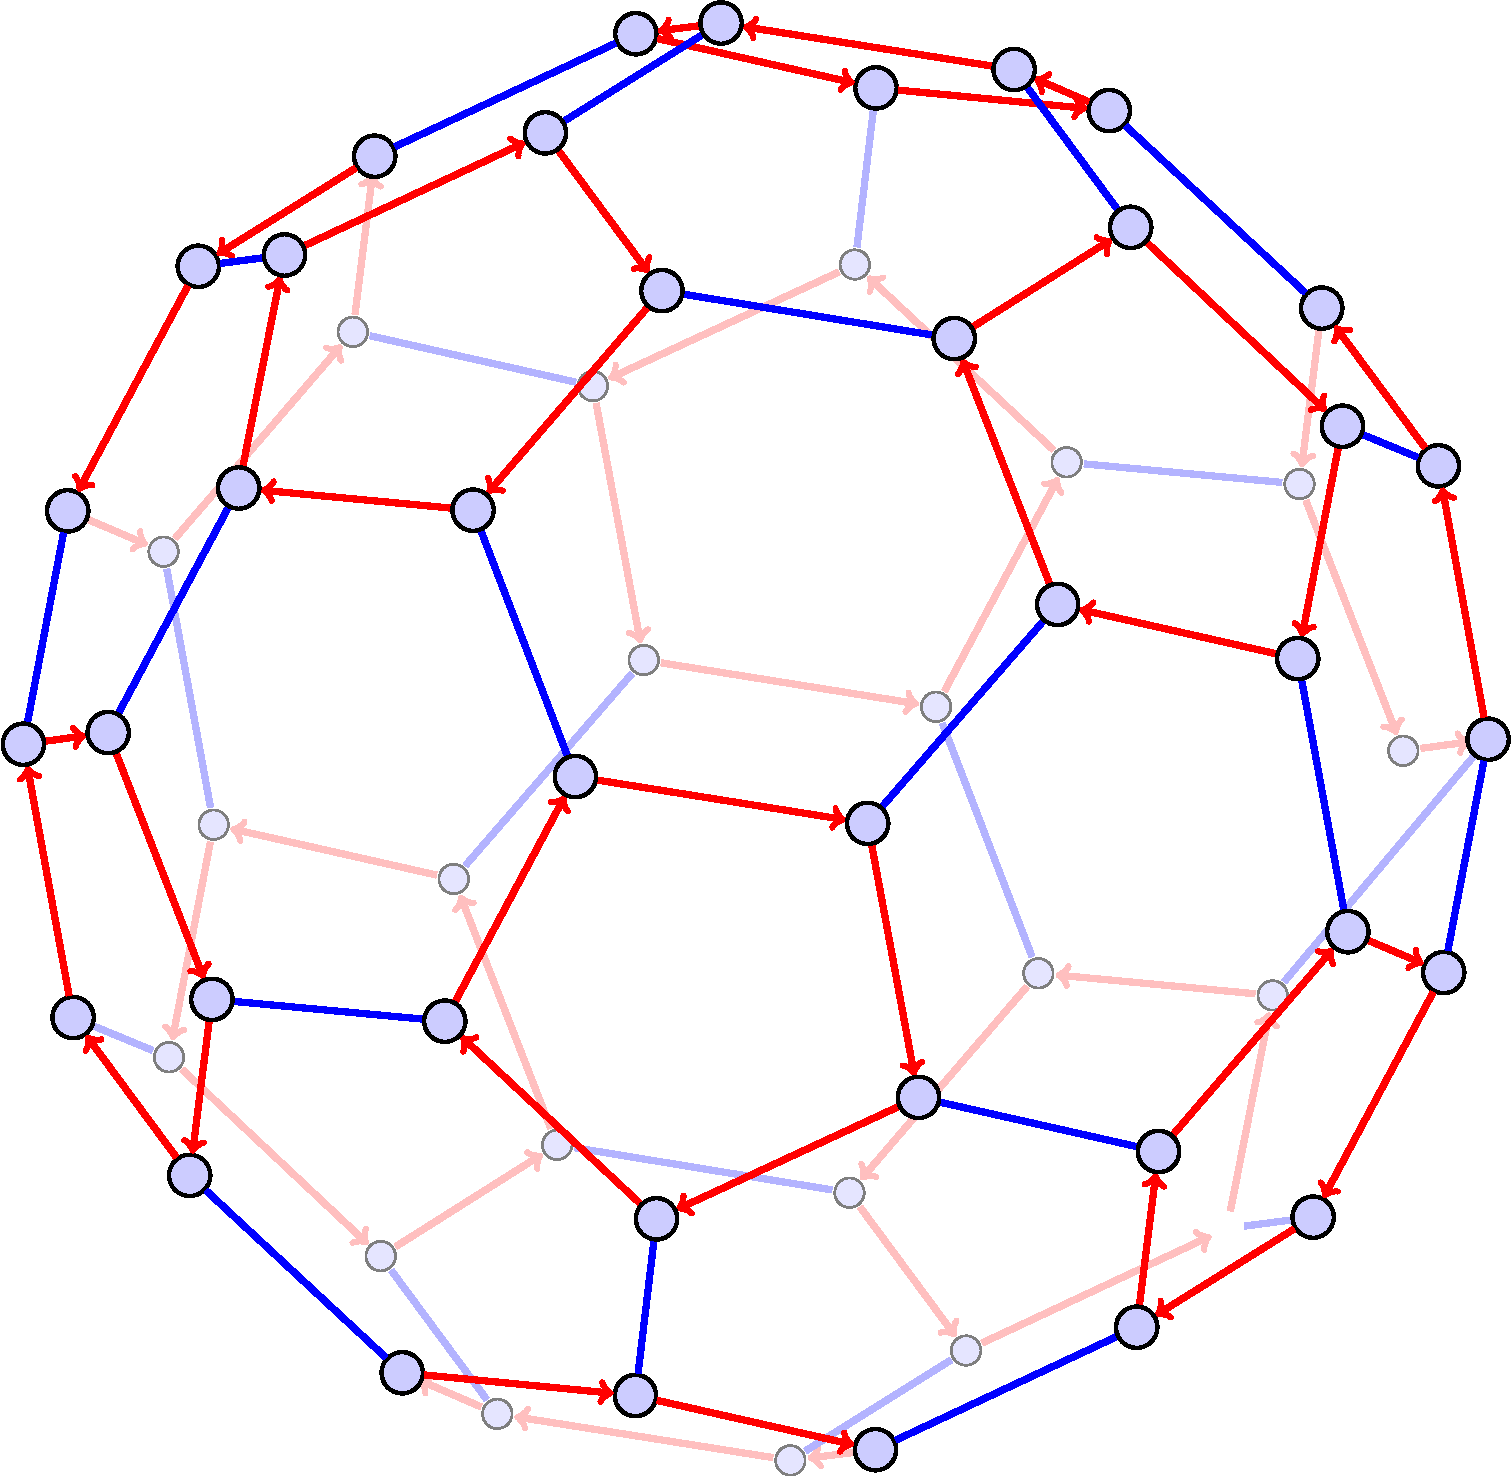
\includegraphics[height=2.5cm]{example/m2.pdf}}
\hspace{4em}
\subcaptionbox{PDF 图像,注意这个图略矮些。如果标题很长的话,它会自动换行\label{fig3}}
{	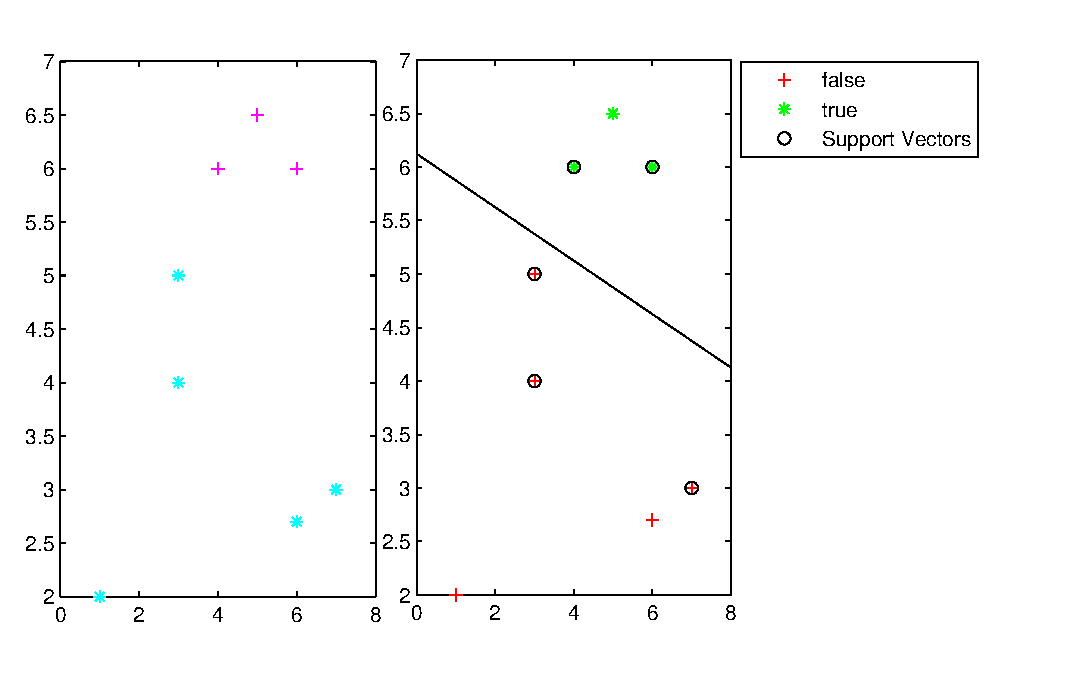
\includegraphics[scale=0.5]{example/figep.eps}}
\bicaption{插入eps和pdf的例子(使用 subcaptionbox 方式)}{An EPS and PDF demo with subcaptionbox}
\label{fig4}
\end{figure}




\section{插入代码}

这里给一个使用listings宏包插入源代码的例子:
\begin{lstlisting}[language={C}, caption={一段C源代码}]
#include <stdio.h>
#include <unistd.h>
#include <sys/types.h>
#include <sys/wait.h>

int main() {
pid_t pid;

switch ((pid = fork())) {
case -1:
printf("fork failed\n");
break;
case 0:
/* child calls exec */
execl("/bin/ls", "ls", "-l", (char*)0);
printf("execl failed\n");
break;
default:
/* parent uses wait to suspend execution until child finishes */
wait((int*)0);
printf("is completed\n");
break;
}

return 0;
}
\end{lstlisting}


\section{参考文献管理}
\label{sec2.5}
\LaTeX 具有将参考文献内容和表现形式分开管理的能力,涉及三个要素:参考文献数据库、参考文献引用格式、在正文中引用参考文献。
这样的流程需要多次编译:
\begin{enumerate}[noitemsep,topsep=0pt,parsep=0pt,partopsep=0pt]
\item 用户将论文中需要引用的参考文献条目,录入纯文本数据库文件(bib文件)。
\item 调用xelatex对论文模板做第一次编译,扫描文中引用的参考文献,生成参考文献入口文件(aux)文件。
\item 调用bibtex,以参考文献格式和入口文件为输入,生成格式化以后的参考文献条目文件(bib)。
\item 再次调用xelatex编译模板,将格式化以后的参考文献条目插入正文。
\end{enumerate}

参考文献数据库(thesis.bib)的条目,可以从Google Scholar搜索引擎\footnote{\url{https://scholar.google.com}}、CiteSeerX搜索引擎\footnote{\url{http://citeseerx.ist.psu.edu}}中查找,文献管理软件Papers\footnote{\url{http://papersapp.com}}、Mendeley\footnote{\url{http://www.mendeley.com}}、JabRef\footnote{\url{http://jabref.sourceforge.net}}也能够输出条目信息。

下面是在Google Scholar上搜索到的一条文献信息,格式是纯文本:

\begin{lstlisting}[caption={从Google Scholar找到的参考文献条目}, label=googlescholar, escapeinside="", numbers=none]
@phdthesis{"白2008信用风险传染模型和信用衍生品的定价",
title={"信用风险传染模型和信用衍生品的定价"},
author={"白云芬"},
year={2008},
school={"上海交通大学"}
} 
\end{lstlisting}

推荐修改后在bib文件中的内容为:

\begin{lstlisting}[caption={修改后的参考文献条目}, label=itemok, escapeinside="", numbers=none]
@phdthesis{bai2008,
title={"信用风险传染模型和信用衍生品的定价"},
author={"白云芬"},
date={2008},
address={"上海"},
school={"上海交通大学"}
} 
\end{lstlisting}

参考文献的引用:
\begin{itemize}
\item 参考文献在正文中被引用,使用命令\verb+\cite{key}+,如\cite{M91}。
\item 参考文献未引用但仍希望列在书末的参考文献中,使用命令\verb+\nocite{key}+,如\verb+\nocite{WI64,G03,D01,JS03}+.
\end{itemize}
\nocite{WI64,G03,D01,JS03}